%
% File: chap01.tex
% Author: Victor F. Brena-Medina
% Description: Introduction chapter where the biology goes.
%
\let\textcircled=\pgftextcircled
\chapter{Results \& Discussion}
\label{chap:results}

\section{Results}
\paragraph{}

The time of computation of different instructions vary slightly. 

At 1.8V Vdd for 180nm SCL PDK, total Read, Compute and Store process time for each instruction containing 4 bit words is as follows:
\begin{itemize}
\item NAND - 3.5ns
\item NOR - 3.5ns
\item XOR - 3.5ns
\item NOT - 3ns
\item Shift Right - 7ns
\item Shift Left - 7ns
\item ADD - 4ns
\item SUB - 5ns
\item WRITE (direct memory access) - 1.5ns
\item READ (direct memory access) - 2ns
\end{itemize}

At 1.8V Vdd for 180nm SCL PDK, the power consumption for the processes containing 4 bit words were as follows:
\begin{itemize}
\item NAND, NOR, XOR NOT, ADD, SUB - 0.402 mW
\item Shift(Both) - 0.583 mW
\end{itemize}

The transient responses were shown for all the operations in Chapter - 4.

\begin{figure}[H]
\centering
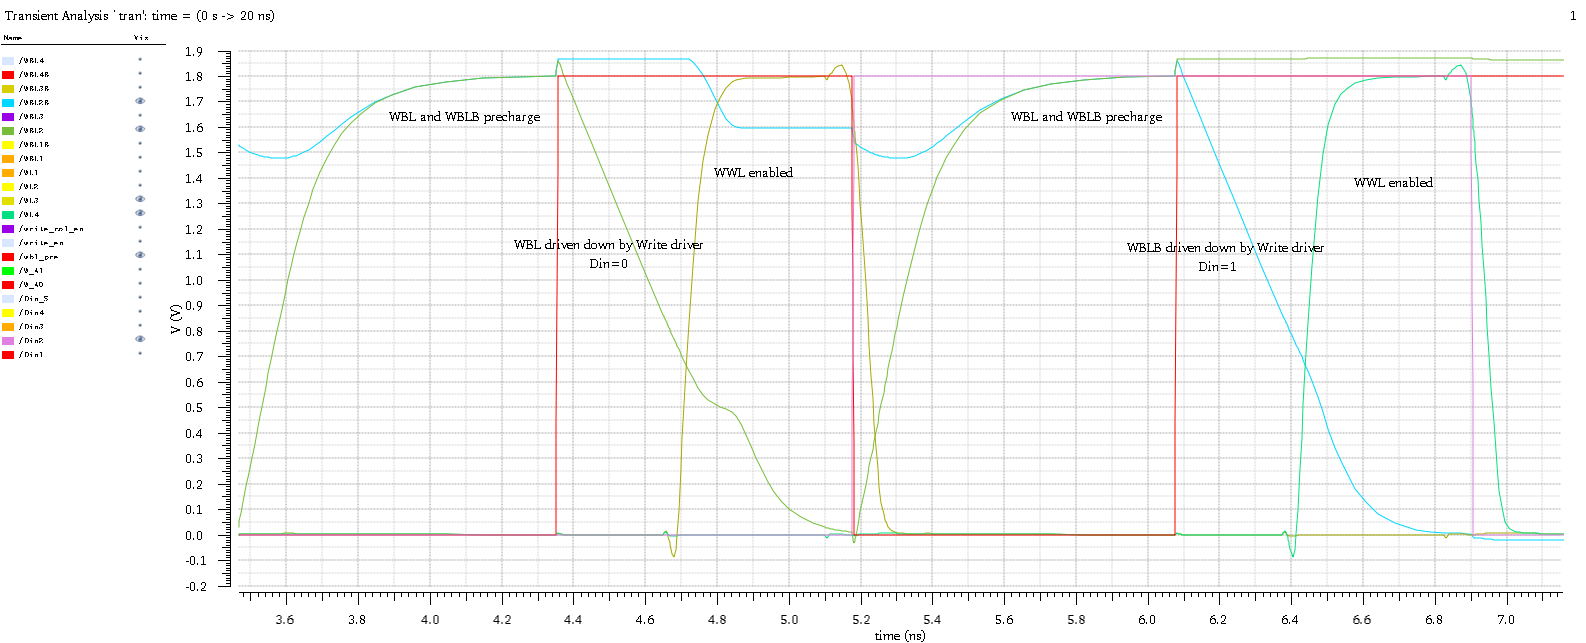
\includegraphics[width=1.0\textwidth]{write_with_peripherals.png}
\caption{Write operation (direct memory access)}
\label{fig:Figure}
\end{figure}

\begin{figure}[H]
\centering
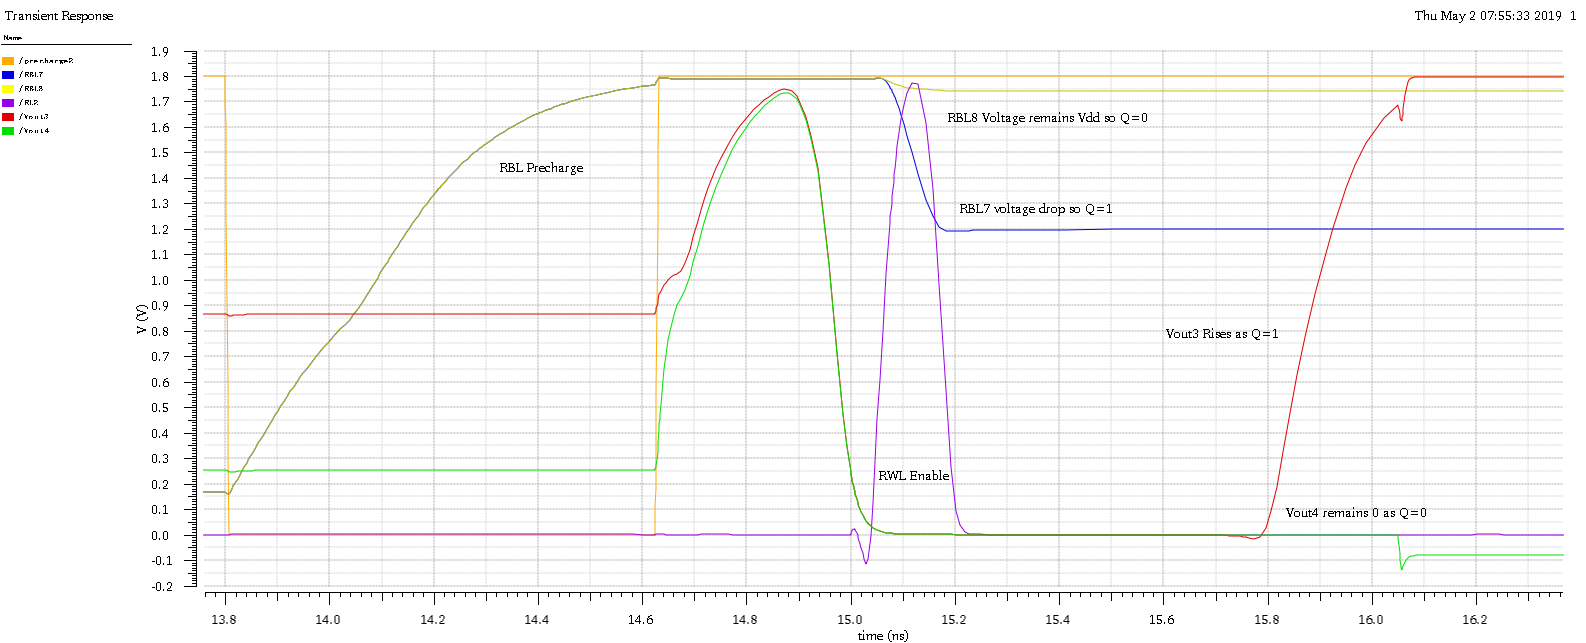
\includegraphics[width=1.0\textwidth]{read_with_peripherals.png}
\caption{Read operation (direct memory access)}
\label{fig:Figure}
\end{figure}

\section{Discussion}
\paragraph{}


After developing the schematic design for the architecture, Layout can be made in order to get more insights into post layout execution issues and also we can have a decent idea about the area efficiency actually achieved. Post Silicon testing or post fabrication testing are indeed essential to get genuine outputs and results of the proposed architecture, and to know how much does this methodology deliver over the conventional ones.

